\chapter{Equipment}\label{chap:equipment}
\begin{figure}[!htb]
\centering
\includegraphics[width=1.0\linewidth]{images/market.jpg}
\end{figure}

\epigraph{\textit{
    I have heard tales that suits of clothing fashioned from metal have even been
    found from time to time. It is generally agreed that these were worn by
    warriors to protect against the blows of enemy weapons. I can only speculate
    that the climate must have been far cooler in those ancient days. Any fool
    that would wear such clothing now would die faster from heat stroke than he
    would have from the weapons of his foes. Still, the idea that there was once
    enough metal in the world to allow such a garment to have been manufactured
    astounds me.\\
    There are even rumors that mounds of steel, silver, and gold lie hidden in
    the deepest tunnels of certain forlorn cities. I have never seen such a thing
    myself, but if such treasures exist, they will reward those who find them most
    handsomely. Those who control such stores of metal can buy food, power,
    influence, and sometimes even the sorcerer-king’s protection.
} }{
    The Wanderer’s Journal
}

\begin{multicols}{2}

\textit{Dark Sun} characters must be well equipped in order to endure the rigors of Athas.
This chapter covers a variety of topics related to mundane equipment that every
hero needs to survive and prosper.

\section{Equipping a Character}
\subsection{Money}
The default money unit is an \textit{Ceramic Piece} or \textit{cp}. This unit can be subdivided in
\textit{Ceramic Bits} (\textit{bit}) and \textit{Lead Bead (bd)}. Larger units are \textit{Silver Pieces} (\textit{sp}) and
\textit{Gold Pieces} (\textit{gp}).\\
\\
10,000 bd = 1,000 bits = 100 cp = 10 sp = 1gp.\\
\\
Ceramics are made from glazed clay and baked in batches once a year in a secure
process supervised by the high templar that supervises the city’s treasury. Bits
are literally one‐tenth parts of a ceramic piece—the ceramic pieces break easily
into ten bits. Some cities’ ceramic pieces have small holes that can be threaded
onto a bracelet or necklace. The lowest unit of Athasian trade is the lead bead
(bd).  In general, the Athasian economy in the cities is relatively stable thanks
to the Merchant Houses. Under normal conditions, supply is ample thanks to the
caravans traveling back and forth between the cities. However, for smaller
communities and trade outposts the price situation on certain goods can sway
drastically. A raider attack or sandstorm can result in lack of necessities such
as food and water, for which people will pay almost any amount of coin. Coins
are not the only means of exchange. Barter and trade in commodities is widespread.

\section{Rarity}\label{sec:equipment-rarity}

When selling an item, your character needs to make
a successful Negotiation check. Use the difficulty set by
the item's rarity (as determined by \tableref{equipment-rarity}).\\
\\
For the cost modifiers of selling an item, please refer to \tableref{trading-modifiers}

\begin{table}[H]
\begin{GenesysTable}{Rarity}{equipment-rarity}{ =l +X}
Rarity & Difficulty\\
0\newline
1      & Simple (-)\\
2\newline
3      & Easy (\difficulty)\\
4\newline
5      & Average (\difficulty\difficulty)\\
6\newline
7      & Hard (\difficulty\difficulty\difficulty)\\
8\newline
9      & Daunting (\difficulty\difficulty\difficulty\difficulty)\\
10     & Formidable (\difficulty\difficulty\difficulty\difficulty\difficulty)\\
\end{GenesysTable}
\end{table}

\begin{table}[H]
\begin{GenesysTable}{Rarity Modifiers}{equipment-rarity-modifiers}{ =l +X}
Rarity Modifiers & Circumstances\\
-1 & Item or resource in complete abundance\\
+0 & Trading Hub\\
+1 & Vassal Village\\
+2 & Small Village\\
+3 & Secret Slave Village\\
+4 & War Zone or Burned Down Village\\
\end{GenesysTable}
\end{table}

\begin{table}[H]
\begin{GenesysTable}{Increased Costs when Trading}{equipment-rarity-costs}{ =l +X}
Rarity Increase & Cost Increase\\
-2              & x0.75\\
-1              & x0.9\\
+0              & x1\\
+1              & x1.5\\
+2              & x2\\
+3              & x3\\
+4 or Higher    & x4\\
\end{GenesysTable}
\end{table}

\section{Item Qualities}\label{sec:item-qualities}
Some variety equipment and depth features to the weapons, special qualities
armor, and that items add your character may encounter. Item qualities are
special rules that can change how the item acts.

Special qualities are generally either passive or active. Passive qualities are
always "on" and require no activation on the part of the user. Active qualities
must be triggered by the user, often by spending one or more \advantage to
activate the effect.

Item qualities usually have a number associated with them. This is their rating.
Ratings affect qualities in different ways, depending on the quality in question.
Active qualities require \advantage\advantage to activate unless otherwise stated
in their description. Active item qualities on weapons can only trigger on a
successful attack, unless specified otherwise.

\subsection{Repairing Gear}\label{sec:repairing-gear}

As a general rule, Athasian items break with can break with spending either
\threat\threat\threat or \despair, instead of only on a \despair. Items with the
\iqtyref{superior} quality or made from metal are exempt from both rules.

\begin{table}[H]
\begin{GenesysTable}{Item Repair}{item-repair}{ =l +l +l}
Repair Required   & Difficulty                                  & Penalty when in use\\
No Repair Needed  & -                                           & -\\
Minor             & \textbf{Easy} (\difficulty)                          & \setback\\
Moderate          & \textbf{Average} (\difficulty\difficulty)            & Increase difficulty by one.\\
Major             & \textbf{Hard} (\difficulty\difficulty\difficulty)    & Unusable.\\
\end{GenesysTable}
\end{table}

\subsection {General Qualities}

\subsubsection{Accurate}
\label{iqty:accurate}
\textbf{Type:} Passive\\
Accurate weapons are easier to aim or wield, whether
through design or technology. For each level of this
quality, the attacker adds \boost to their combat checks
while using this weapon.

\subsubsection{Auto-Fire}
\label{iqty:autofire}
\textbf{Type:} Active\\
A weapon with Auto-fire can be set to shoot in rapid
succession and potentially spray an area with bolts,
flechettes, slugs, or other types of projectiles. The
advantage in using Auto-fire is that it has the chance to hit
multiple targets or to hit a single target multiple times.
As attacking with a weapon on Auto-fire is generally
less accurate, the attacker must increase the difficulty
of the combat check by \difficulty. The user may choose not
to use the Auto-fire quality on a weapon; in this case,
they cannot trigger the quality but also do not suffer
the aforementioned penalty.

If the attack hits, the attacker can trigger Auto-fire
by spending \advantage\advantage. Auto-fire can be triggered multiple
times. Each time the attacker triggers Auto-fire, it deals
an additional hit to the target. Each of these counts as an
additional hit from that weapon, and each hit deals base
damage plus the number of \success on the check.
These additional hits can be allocated to the original
target, or to other targets within range of the weapon.
If the attacker wishes to hit multiple targets, they must
decide to do so before making the check. Furthermore, if
they wish to hit multiple targets, their initial target must
always be the target with the highest difficulty and highest
defense (if this is two separate targets, the GM chooses
which is the initial target). The initial hit must always be
against the initial target. Subsequent hits generated can
be allocated to any of the other designated targets.
Auto-fire weapons can also activate one Critical Injury for
each hit generated on the attack, per the normal rules; the
Critical Injury must be applied to the target of the specific
hit.


\subsubsection{Backup}
\label{iqty:backup}
\textbf{Type:} Passive\\
A backup weapon does not need to be drawn. It could for example be a spiked gauntlet that is
already worn.

\subsubsection{Blast}
\label{iqty:blast}
\textbf{Type:} Active\\
The weapon has a large spread, an explosive blast, or
a similar area of effect, like a detonated grenade or a
warhead fired from a missile launcher. If the attack is
successful and Blast activates, each character (friend
or foe) engaged with the original target suffers a hit
dealing damage equal to the Blast quality’s rating, plus
damage equal to the total \success scored on the check.
In a relatively small and enclosed area, the Game Master
might decide that everyone in the room suffers damage.
If the Blast quality doesn’t activate, the ordnance still
detonates, but bad luck or poor aim on the part of the
firer (or quick reactions on the part of the targets) means
the explosion may not catch anyone else in its radius.
However, the user may also trigger Blast if the attack
misses by spending \advantage\advantage\advantage. In
this case, the original target and every target engaged
with the original target suffers a hit dealing damage
equal to the Blast rating of the weapon.

\subsubsection{Brace}
\label{iqty:brace}
\textbf{Type:} Passive\\
When attacking an engaged mounted enemy
which engaged you after the end of your last round, the
Aim maneuver grants \boost\boost instead of \boost.

\subsubsection{Burn}
\label{iqty:burn}
\textbf{Type:} Active\\
Weapons with Burn inflict damage over time. When
Burn is triggered, one target hit by the attack continues
to suffer the weapon’s base damage each round for a
number of rounds equal to the weapon’s Burn rating.
Apply damage at the start of each of the target’s turns.
If multiple targets suffer hits from a weapon with Burn,
the quality may be triggered multiple times, affecting a
different target each time.
A victim might be able to stop the damage by per-
forming an action to roll around and make a Coordination check.
The difficulty is Average (\difficulty\difficulty) on hard
surfaces such as the floor of a building, or an Easy (\difficulty)
on grass or soft ground. Jumping into a body of water
stops the damage immediately. Both situations assume
the flame is from actual combustion rather than a
chemical reaction. With the latter, there is usually little
the victim can do.

\subsubsection{Concealable}
\label{iqty:concealable}
\textbf{Type:} Passive\\
These weapons can be easily concealed. An
observer adds \setback to Perception/Vigilance
check to find the weapon.

\subsubsection{Concussive}
\label{iqty:concussive}
\textbf{Type:} Active\\
The weapon’s attack can leave the target shell-shocked
from mighty blows or punishing shock waves, unable
to perform any but the most basic actions. When Concussive
is triggered, one target hit by the attack is staggered
(see Genesys pg. 114) for a number of rounds equal to
the weapon’s Concussive rating. A staggered target cannot
perform actions. If multiple targets suffer hits from
a weapon with Concussive, the quality may be triggered
multiple times, affecting a different target each time.

\subsubsection{Cortosis}
\label{iqty:cortosis}
\textbf{Type:} Passive\\
Weapons with the Cortosis quality are immune to
the Sunder quality. Armor with the Cortosis quality
makes the w earer’s soak immune to the Pierce and
Breach qualities.

\subsubsection{Cumbersome}
\label{iqty:cumbersome}
\textbf{Type:} Passive\\
A Cumbersome weapon is large, unwieldy, awkward,
or heavy. To wield a Cumbersome weapon properly,
the character needs a Brawn characteristic equal to
or greater than the weapon’s Cumbersome rating. For
each point of Brawn by which the character is deficient,
they must increase the difficulty of all checks made
while using the weapon by one.

\subsubsection{Defensive}
\label{iqty:defensive}
\textbf{Type:} Passive\\
An item with the Defensive quality increases the user’s
melee defense by its Defensive rating.

\subsubsection{Deflection}
\label{iqty:deflection}
\textbf{Type:} Passive\\
An item with the Deflection quality increases the user’s
ranged defense by its Deflection rating.

\subsubsection{Disarm}
\label{iqty:disarm}
\textbf{Type:} Active\\
By spending \advantage\advantage, you can have the opponent
drop his weapon.

\subsubsection{Disorient}
\label{iqty:disorient}
\textbf{Type:} Active\\
A weapon with Disorient can daze an opponent. When
Disorient is triggered, one target hit by the attack is
disoriented (see Genesys pg. 114) for a number of rounds equal
to the weapon’s Disorient rating. A disoriented target
adds \setback to all skill checks they perform. If
multiple targets suffer hits from a weapon with Disorient,
the quality may be triggered multiple times, affecting a
different target each time.

\subsubsection{Ensnare}
\label{iqty:ensnare}
\textbf{Type:} Active\\
A weapon with Ensnare binds a foe and restricts their
movements. When Ensnare is triggered, one target hit
by the attack becomes immobilized (see Genesys pg. 114)
for a number of rounds equal to the weapon’s Ensnare
rating. An immobilized target cannot perform maneuvers.
If multiple targets suffer hits from a weapon with
Ensnare, the quality may be triggered multiple times,
affecting a different target each time.
An Ensnared target may perform an action to attempt
a Hard (\difficulty\difficulty\difficulty) Athletics
check on their turn to break free from the effect.

\subsubsection{Flimsy}
\label{iqty:flimsy}
\textbf{Type:} Passive\\
Flimsy items lose any soak value they have when
targeted by weapons with a Pierce rating.

\subsubsection{Fragile}
\label{iqty:fragile}
\textbf{Type:} Passive\\
The item only has 2 health levels as opposed to the
normal 3 (moderate and major only).

\subsubsection{Inaccurate}
\label{iqty:inaccurate}
\textbf{Type:} Passive\\
Inaccurate weapons are less likely to be accurate or pre-
cise. When making an attack with an Inaccurate weapon,
add \setback to the check equal to the Inaccurate rating.

\subsubsection{Inferior}
\label{iqty:inferior}
\textbf{Type:} Passive\\
An Inferior item is a lackluster example of its kind, repre-
senting shoddy and poor craftsmanship. An Inferior item
generates automatic \threat on all checks related to its use.

\subsubsection{Knockdown}
\label{iqty:knockdown}
\textbf{Type:} Passive\\
When Knockdown is triggered, one target hit by the
attack is knocked prone. If multiple targets suffer hits
from a weapon with Knockdown, the quality may be triggered
multiple times, affecting a different target each time.
Unless specified otherwise, Knockdown requires \advantage
\advantage to trigger, plus one additional \advantage per
silhouette of the target beyond 1.

\subsubsection{Limited Ammo}
\label{iqty:limitedammo}
\textbf{Type:} Passive\\
Some weapons fire particularly large or complex
projectiles that cost lots of money. Other weapons are
expendable weapons like grenades that, once used, are
destroyed. A weapon with the Limited Ammo quality
may be used to make a number of attacks equal to its
Limited Ammo rating before it must be reloaded with a
maneuver. In addition, each shot expends one of a
limited number of rounds of ammo; more ammo must be
purchased or obtained before anyone fires the weapon
again. This also applies to grenades and other "one-use"
weapons that have the Limited Ammo 1 quality (here,
your character is not "reloading" the grenade, but
drawing another to use—mechanically, they are equivalent).

\subsubsection{Noisy}
\label{iqty:noisy}
\textbf{Type:} Passive\\
Items with the Noisy quality bestow \setback on stealth
checks made while the item is in use. These \setback are
cumulative if multiple noisy items are carried at once.

\subsubsection{Pierce}
\label{iqty:pierce}
\textbf{Type:} Passive\\
Any hits from this weapon ignore a number of points
point of soak equal to the weapon’s Pierce rating. If the
weapon has more ranks of Pierce than the target’s total
soak, it completely ignores the target’s soak. For example,
Pierce 3 against a soak of 2 ignores two points of
soak, but the extra point of Pierce has no further effect.

\subsubsection{Prepare}
\label{iqty:prepare}
\textbf{Type:} Passive\\
Items with this quality require time to set up before
being used. The user must perform a number of
preparation maneuvers equal to the item’s Prepare
rating before using the item (if the item is a weapon,
"using" it would be making attacks with the weapon).
At your GM’s discretion, moving with the item, being
knocked prone with the item, or other disruptions may
require the user to perform the preparation maneuvers
again before using the item.

\subsubsection{Reach}
\label{iqty:reach}
\textbf{Type:} Passive\\
Disengaging from an opponent wielding a melee weapon
with this quality requires 2 manoeuvres rather than the
normal 1.


\subsubsection{Reinforced}
\label{iqty:reinforced}
\textbf{Type:} Passive\\
Weapons or items with the Reinforced quality are
immune to the Sunder quality. Armor with the
Reinforced quality make the wearer's soak immune to
the Pierce and Breach qualities.

\subsubsection{Restrictive}
\label{iqty:restrictive}
\textbf{Type:} Passive\\
Restrictive items are difficult to move in
when worn. Characters wearing restrictive armor
upgrade the difficulty of Agility based checks once.

\subsubsection{Returning}
\label{iqty:returning}
\textbf{Type:} Active\\
Returning weapons are throwing weapons which will return
to the wielder at the end of the wielders turn if thrown
correctly and the wielder is a bit lucky.
Returning costs and \advantage.

\subsubsection{Slow-Firing}
\label{iqty:slowfiring}
\textbf{Type:} Passive\\
Slow-Firing weapons tend to deal incredible damage,
but need time to recharge or cool down between shots.
A weapon’s Slow-Firing rating dictates the number of
rounds that must pass before the weapon can be fired
again after attacking. For example, a heavy laser cannon
with Slow-Firing 2 must wait two rounds after being
fired before it can be fired again.

\subsubsection{Solid}
\label{iqty:solid}
\textbf{Type:} Passive\\
Solid items resist Pierce up to their rating. If the
Pierce of an attack against an object surpasses its Solid
rating, the Solid quality is ignored.

\subsubsection{Stun}
\label{iqty:stundamage}
\textbf{Type:} Active\\
A weapon with this quality can deal strain damage.
When the Stun quality is activated, it inflicts strain
equal to the weapon's Stun rating. Since this is
strain, not strain \textit{damage}, it is not reduced
by a target’s soak.

\subsubsection{Stun Damage}
\label{iqty:stun}
\textbf{Type:} Passive\\
A weapon with this quality can only deal strain damage
(damage applied to the target’s strain threshold).
Because this is strain \textit{damage}, not strain,
it is still reduced by a target’s soak.

\subsubsection{Sunder}
\label{iqty:sunder}
\textbf{Type:} Active\\
When activating Sunder, the attacker chooses one item
openly wielded by the target (such as a weapon, shield, or
item on a belt). That item is damaged one step: to minor
if undamaged, from minor to moderate, or from moderate
to major. If an item already suffering major damage is
the target of a successful Sunder, it is destroyed.
Sunder requires \advantage to activate, and may be activated
even if the attack is unsuccessful. Sunder may be activated
multiple times in the same attack, but each activation
must be applied to the same item, potentially taking
it from undamaged to destroyed in a single attack.

\subsubsection{Superior}
\label{iqty:superior}
\textbf{Type:} Passive\\
A Superior item is a sterling example of its kind,
representing masterful craftsmanship. A Superior item
generates automatic \advantage on all checks related to
its use. In addition, it can only break on a \despair,
instead of both \threat\threat\threat or a \despair.

\subsubsection{Thrown}
\label{iqty:thrown}
\textbf{Type:} Passive\\
These melee weapons can also be thrown up to
short range using Ranged skill. When thrown, they
inflict the same damage as if used into melee and gain
the Limited Ammo 1 quality.

\subsubsection{Unwieldy}
\label{iqty:unwieldy}
\textbf{Type:} Passive\\
An Unwieldy weapon is a weapon that can be particularly awkward to use for those
without impressive dexterity and hand-eye coordination. To wield an Unwieldy
weapon properly, the character needs an Agility characteristic equal to or
greater than the weapon's Unwieldy rating. For each point of Agility by which
the character is deficient, they must increase the difficulty of all checks
made while using the weapon by one.

\subsubsection{Vicious}
\label{iqty:vicious}
\textbf{Type:} Passive\\
When an attack with this weapon results in a Critical
Injury or Hit, the character adds ten times the Vicious rat-
ing to the Critical roll. With Vicious 3, for example, you
would add +30 to the resulting Critical Injury or Hit result.


\end{multicols}
\FloatBarrier
\section{Items}\label{sec:items}

\begin{figure}[!htb]
\centering
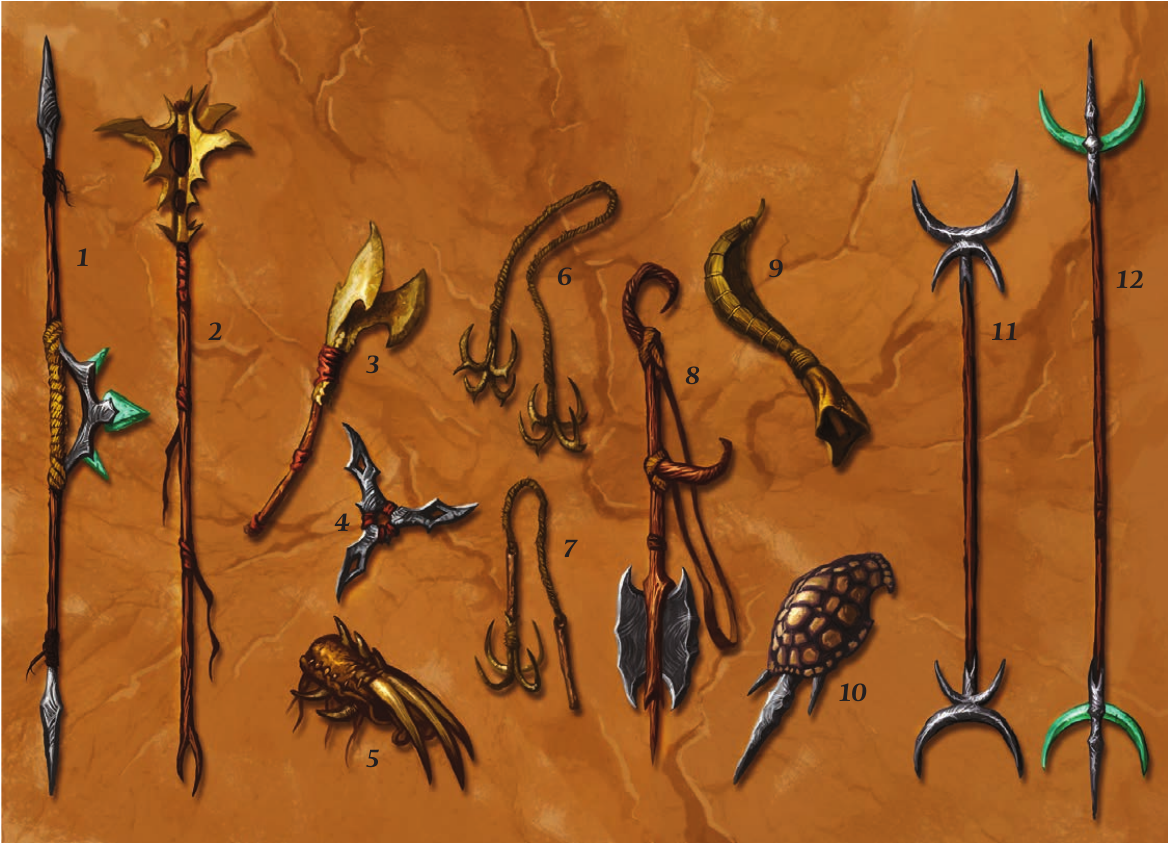
\includegraphics[width=0.8\linewidth]{images/weapons.png}
\captionof{figure}{
    1.  \nameref{itmmlee:dragonpaw};
    2.  \nameref{itmmlee:trikal};
    3.  \nameref{itmmlee:carrikal};
    4.  \nameref{itmrng:catkcha};
    5.  \nameref{itmmlee:wristrazors};
    6.  \nameref{itmmlee:cahulaks};
    7.  \nameref{itmmlee:alhulak};
    8.  \nameref{itmmlee:gouge};
    9.  \nameref{itmrng:dejada};
    10. \nameref{itmmlee:tortoiseblade};
    11. \nameref{itmmlee:lotulis};
    12. \nameref{itmmlee:gythka} }
\end{figure}

%TODO: Rebalance
\subsection{Melee Weapons}

\begin{table*}[!htb]
\centering
\small\caption{Brawl Weapons}
\begin{GenesysTable}{l l l l l l X}
Name                            & Dam & Crit & Encum & Price   & Rarity & Special     \\
\nameref{itmmlee:punchik}       & +1  & 3    & 1     & 75 cp   & 0      & \nameref{iqty:fragile}, \nameref{iqty:pierce} 1 \\
\nameref{itmmlee:talid}         & +0  & 4    & 1     & 60 cp   & 2      & \nameref{iqty:fragile}, \nameref{iqty:backup}, \nameref{iqty:disorient} 3 \\
\nameref{itmmlee:wristrazors}   & +1  & 3    & 0     & 30 cp   & 2      & \nameref{iqty:fragile}, \nameref{iqty:backup}, \nameref{iqty:pierce} 2 \\
\nameref{itmmlee:net}           & -1  & -    & 1     & 30 cp   & 2      & \nameref{iqty:ensnare} 4, \nameref{iqty:thrown} \\
\nameref{itmmlee:whip}          & +1  & 4    & 0     & 30 cp   & 2      & \nameref{iqty:ensnare} 2, \nameref{iqty:stundamage} \\
\nameref{itmmlee:tortoiseblade} & +0  & 6    & 1     & 90 cp   & 3      & \nameref{iqty:fragile}, \nameref{iqty:defensive} 1, \nameref{iqty:inaccurate} 2, \nameref{iqty:pierce} 1 \\
\end{GenesysTable}
\end{table*}

\begin{table*}[!htb]
\centering
\small\caption{Light Melee Weapons}
\begin{GenesysTable}{l l l l l l X}
Name                         & Dam & Crit & Encum & Price    & Rarity & Special  \\
\nameref{itmmlee:knife}      & +1  & 3    & 1     & 25 cp    & 1   & \nameref{iqty:fragile}, \nameref{iqty:thrown} \\
\nameref{itmmlee:buckler}    & +0  & 6    & 1     & 40 cp    & 0   & \nameref{iqty:defensive} 1, \nameref{iqty:inaccurate} 1 \\
\nameref{itmmlee:club}       & +2  & 5    & 2     & 15 cp    & 1   & \nameref{iqty:disorient} 4 \\
\nameref{itmmlee:shortspear} & +2  & 4    & 2     & 90 cp    & 1   & \nameref{iqty:fragile}, \nameref{iqty:accurate} 1, \nameref{iqty:defensive} 1, \nameref{iqty:thrown} \\
\nameref{itmmlee:carrikal}   & +3  & 3    & 2     & 150 cp   & 3   & \nameref{iqty:fragile}, \nameref{iqty:vicious} 1 \\
\nameref{itmmlee:alhulak}    & +2  & 4    & 2     & 90 cp    & 2   & \nameref{iqty:fragile}, \nameref{iqty:disarm} \\
\nameref{itmmlee:macuahuitl} & +1  & 2    & 2     & 200 cp   & 5   & \nameref{iqty:fragile}, \nameref{iqty:vicious} 1 \\
\end{GenesysTable}
\end{table*}

\begin{table*}[!htb]
\small\caption{Heavy Melee Weapons}
\centering
\begin{GenesysTable}{l l l l l l X}
Name                          & Dam & Crit  & Encum & Price     & Rarity & Special     \\
\nameref{itmmlee:shield}      & +0  & 6     & 2     & 80 cp     & 1     & \nameref{iqty:defensive} 1, \nameref{iqty:deflection} 1, \nameref{iqty:inaccurate} 1, \nameref{iqty:knockdown} \\
\nameref{itmmlee:gouge}       & +4  & 2     & 3     & 300 cp    & 4     & \nameref{iqty:fragile}, \nameref{iqty:disorient} 2, \nameref{iqty:unwieldy} 3 \\
\nameref{itmmlee:longspear}   & +3  & 4     & 3     & 250 cp    & 2     & \nameref{iqty:fragile}, \nameref{iqty:reach}, \nameref{iqty:defensive} 1, \nameref{iqty:pierce} 1 \\
\nameref{itmmlee:lotulis}     & +4  & 3     & 4     & 300 cp    & 4     & \nameref{iqty:fragile}, \nameref{iqty:cumbersome} 3, \nameref{iqty:pierce} 1, \nameref{iqty:sunder} \\
\nameref{itmmlee:trikal}      & +3  & 3     & 5     & 250 cp    & 2     & \nameref{iqty:fragile}, \nameref{iqty:defensive} 1, \nameref{iqty:pierce} 3 \\
\nameref{itmmlee:cahulaks}    & +2  & 3     & 2     & 275 cp    & 2     & \nameref{iqty:fragile}, \nameref{iqty:thrown}, \nameref{iqty:reach}, \nameref{iqty:unwieldy} 3 \\
\nameref{itmmlee:dragonpaw}   & +2  & 4     & 2     & 275 cp    & 2     & \nameref{iqty:fragile}, \nameref{iqty:defensive} 1, \nameref{iqty:accurate} 1, \nameref{iqty:disarm} \\
\nameref{itmmlee:gythka}      & +2  & 4     & 2     & 275 cp    & 2     & \nameref{iqty:fragile}, \nameref{iqty:thrown}, \nameref{iqty:vicious} 1 \\
\end{GenesysTable}
\end{table*}
\begin{multicols}{2}

\subsubsection{Alhulak}
\label{itmmlee:alhulak}
This weapon is an unusual flail. A short length of rope separates
a four-bladed, hafted grappling hook from the handle.

\subsubsection{Buckler}
\label{itmmlee:buckler}
Whether crafted from wood, chitin, or hide, shields are
common among warriors of all cultures and skill levels for
a simple reason: they keep you alive. The utility of a shield
for blocking and parrying blows cannot be overstated. While
an important part in every warriors defence, the scorching sun
makes carrying a large shield impracticle and thus use medium
shields or even bucklers.

\subsubsection{Cahulaks}
\label{itmmlee:cahulaks}
This double weapon features two four-
bladed, hafted heads separated by a length of rope.
The secondary end is light enough to be used as an
off-hand weapon. When one end of this weapon is
held by the haft, the rope is long enough to grant the
other end reach. The entire weapon can be thrown.

\subsubsection{Carrikal}
\label{itmmlee:carrikal}
This axe has two forward-facing blades carved from the front
of a large jawbone, commonly that of a mekillot.

\subsubsection{Club}
\label{itmmlee:club}
This weapon is usually just a shaped piece of wood, sometimes
with a few stone or obsidian shards embedded in it.

\subsubsection{Dragon Paw}
\label{itmmlee:dragonpaw}
Short blades attach to either end
of this staff. In the center of this double weapon is a
guard with a protruding blade perpendicular to the
staff. The light, middle blade (which serves as the
off-hand end) can be used for quick jabs, ideal for a
warrior with a roguish bent.

\subsubsection{Gouge}
\label{itmmlee:gouge}
This spadelike weapon has a long haft with a handle on the end. The head
is a wide, double-edged blade with a stabbing point at the top. Some
gouges are fitted with a strap or a harness, making the weapon easier
to carry.

\subsubsection{Gythka}
\label{itmmlee:gythka}
Each end of this thri-kreen staff has a
small, crescent-shaped blade with a centered stabbing
tine. The secondary end of this double weapon is light
enough to be used as an off-hand weapon. A gythka
can be thrown like a javelin.

\subsubsection{Knife}
\label{itmmlee:knife}
A dagger has an obsidian blade that is about 30 cm in length.

\subsubsection{Long Spear}
\label{itmmlee:longspear}
Although a simple weapon, a spear is easy to wield and
allows the user to keep some distance from an oppo-
nent. Hence, spears don’t have very high damage, but
the Accurate 1 quality represents their ease of use. In
addition, the Defensive 1 quality represents their use-
fulness at keeping someone at arms’ reach.

\subsubsection{Lotulis}
\label{itmmlee:lotulis}
This short-staffed double weapon sports outward-pointing,
barbed crescent blades on each end.

\subsubsection{Macuahuitl}
\label{itmmlee:macuahuitl}
A macuahuitl is a wooden club with obsidian blades. Its sides
are embedded with prismatic blades traditionally made from
obsidian. The macuahuitl was a standard close combat weapon.

\subsubsection{Net}
\label{itmmlee:net}
A net is a web of rope or cord fitted with heavy weights.

\subsubsection{Punchik}
\label{itmmlee:punchik}
Punhicks are often little more than a wooden or bone
bar with a large obsidian spike attached to it, with the spike
coming out between your fingers. They are the smallest, simplest,
and easiest to conceal type of brawl weapon. Due to their
small size, punchiks are quite easy to conceal in a pocket,
pouch, or compartment in easy reach until they're needed. Add
\setback to a character's Perception check when attempting to
find a punchik on a person's body.

\subsubsection{Shield}
\label{itmmlee:shield}
Whether crafted from wood, chitin, or hide, shields are
common among warriors of all cultures and skill levels for
a simple reason: they keep you alive. The utility of a shield
for blocking and parrying blows cannot be overstated. While
an important part in every warriors defence, the scorching sun
makes carrying a large shield impracticle and thus use medium
shields or even bucklers.

\subsubsection{Short Spear}
\label{itmmlee:shortspear}
Although a simple weapon, a spear is easy to wield and
allows the user to keep some distance from an oppo-
nent. Hence, spears don’t have very high damage, but
the Accurate 1 quality represents their ease of use. In
addition, the Defensive 1 quality represents their use-
fulness at keeping someone at arms’ reach.

\subsubsection{Talid}
\label{itmmlee:talid}
Made from leather, chitin, and bone, this spiked
"gladiator's gauntlet" augments unarmed attacks.

\subsubsection{Tortoise Blade}
\label{itmmlee:tortoiseblade}
This bony or chitinous plate is affixed with a short
blade that points forward from the wielder's hand.

\subsubsection{Trikal}
\label{itmmlee:trikal}
This polearm projects three blades symmetrically lengthwise
from its haft. A trikal is equivalent to a halberd.

\subsubsection{Whip}
\label{itmmlee:whip}
Although a whip is impractical as a weapon
in most circumstances, some opponents are prone
to underestimating the wielder of a whip, which can
lead them to attack rashly or make other mistakes.

\subsubsection{Wrist Razors}
\label{itmmlee:wristrazors}
This weapon consists of three sharp blades that protrude from
a sturdy bracer, freeing the wielder's hand. A shield cannot
be worn on the same arm as wrist razors. Wrist razors do not
need to be drawn, nor do they need to be sheathed for the
wielder to use the hand the razors are on

\end{multicols}

\hrulefill
\subsection{Ranged Weapons}

\begin{table*}[!htb]
\begin{GenesysTable}{Ranged Weapons}{ranged-weapons}{ =l +l +l +l +l +l +l +X}
Name                      & Dam & Crit & Range  & Encum & Price    & Rarity & Special \\
\nameref{itmrng:blowgun}  & 6   & 3    & Short  & 2     & 275 cp   & 3      & \iqtyref{limitedammo} 1\\
\nameref{itmrng:bolas}    & +0  & -    & Short  & 1/3   & 20 cp    & 2      & \iqtyref{ensnare} 3, \iqtyref{knockdown}, \iqtyref{limitedammo} 1 \\
\nameref{itmrng:catkcha}  & +2  & 4    & Short  & 1     & 275 cp   & 4      & \iqtyref{unwieldy} 3, \iqtyref{returning}, \iqtyref{limitedammo} 1 \\
\nameref{itmrng:javelin}  & +2  & 3    & Short  & 1/3   & 40 cp    & 1      & \iqtyref{accurate} 1, \iqtyref{pierce} 1, \iqtyref{limitedammo} 1 \\
\nameref{itmrng:dejada}   & 5   & 3    & Medium & 2     & 275 cp   & 2      & \iqtyref{unwieldy} 2, \iqtyref{concussive} \\
\nameref{itmrng:shortbow} & 7   & 3    & Medium & 2     & 275 cp   & 3      & \iqtyref{unwieldy} 2 \\
\nameref{itmrng:longbow}  & 8   & 3    & Long   & 2     & 275 cp   & 5      & \iqtyref{unwieldy} 3 \\
\end{GenesysTable}
\end{table*}
\begin{multicols}{2}

\subsubsection{Blow Gun}
\label{itmrng:blowgun}
Blowguns are generally used to deliver debilitating (but rarely fatal) poisons from a distance. They are nearly silent when fired.

\subsubsection{Bolas}
\label{itmrng:bolas}
A bola consists of a couple of round stones joined together by a strong string of rope. Skilled throwers can use them to catch or trip prey from a distance.

\subsubsection{Catkcha}
\label{itmrng:catkcha}
This throwing wedge, often shaped from crystal or obsidian, is a thri-kreen invention. It returns to a proficient wielder’s hand after the ranged attack is resolved.

\subsubsection{Dejada}
\label{itmrng:dejada}
A long, scooped basket fitted to a glove-like bracer, the dejada is used to hurl projectiles. Ammunition can be a fist-sized stone, but the weapon is also used to extend the range of alchemical mixtures.

\subsubsection{Javelin}
\label{itmrng:javelin}
A javelin is a thin throwing spear.

\subsubsection{Long Bow}
\label{itmrng:longbow}
At almost 5 feet in height, a longbow is made up of one solid piece of carefully curved wood.

\subsubsection{Short Bow}
\label{itmrng:shortbow}
A shortbow is made up of one piece of wood, about 3 feet in length.

\end{multicols}

\hrulefill
\subsection{Armour}

\begin{table*}[!htb]
\begin{GenesysTable}{Armour}{armour}{ =l +l +l +l +l +l +l +X}
Name                                    & Defense   & Soak  & Encum & Price     & Rarity    & Slots & Special  \\
\nameref{itmamr:heavyrobes}             & 1         & +0    & 1     & 70cp       & 1         & 1     & \iqtyref{concealable}\\
\nameref{itmamr:padded}                 & 1         & +0    & 2     & 50cp       & 2         & 0     & \\
\nameref{itmamr:crodluleather}          & 0         & +1    & 2     & 100cp      & 1         & 1     & \iqtyref{fragile} \\
\nameref{itmamr:baazragleather}         & 0         & +1    & 2     & 300cp      & 5         & 1     & \iqtyref{fragile}, \iqtyref{concealable}\\
\nameref{itmamr:kankhide}               & 1         & +1    & 2     & 450cp      & 3         & 1     & \iqtyref{fragile} \\
%\nameref{itmamr:brohghide}              & 1         & +1    & 2     & 250cp      & 3         & 1     & \iqtyref{fragile} \\
\nameref{itmamr:reaperchitin}           & 0         & +2    & 3     & 600cp      & 4         & 2     & \iqtyref{fragile}, \iqtyref{solid} 1 \\
%\nameref{itmamr:kreenchitin}            & 0         & +2    & 3     & 500cp      & 4         & 1     & \iqtyref{fragile}, \iqtyref{solid} 1 \\
\nameref{itmamr:anakoreshell}           & 1         & +2    & 3     & 1000cp     & 5         & 1     & \iqtyref{fragile}, \iqtyref{noisy}, \iqtyref{solid} 2 \\
%\nameref{itmamr:inixshell}              & 1         & +2    & 3     & 1000cp     & 5         & 3     & \iqtyref{fragile}, \iqtyref{noisy}, \iqtyref{solid} 2 \\
\nameref{itmamr:braxatbreastplate}      & 1         & +2    & 3     & 1200cp     & 6         & 1     & \iqtyref{fragile}\\
\nameref{itmamr:braxathalfplate}        & 2         & +3    & 4     & 6000cp    & 7         & 2     & \iqtyref{fragile}, \iqtyref{restrictive}, \iqtyref{solid} 2 \\
\nameref{itmamr:braxatfullplate}        & 3         & +3    & 5     & 10000cp   & 8         & 2     & \iqtyref{fragile}, \iqtyref{restrictive}, \iqtyref{solid} 3 \\
\nameref{itmamr:mekillotbreastplate}    & 1         & +2    & 3     & 1500cp    & 6         & 2     & \iqtyref{noisy},   \iqtyref{reinforced}\\
\nameref{itmamr:mekillothalfplate}      & 1         & +3    & 4     & 5000cp    & 7         & 2     & \iqtyref{noisy},   \iqtyref{reinforced}, \iqtyref{solid} 2 \\
\nameref{itmamr:mekillotfullplate}      & 2         & +3    & 5     & 8000cp    & 8         & 2     & \iqtyref{noisy},   \iqtyref{reinforced}, \iqtyref{solid} 3 \\
\end{GenesysTable}
\end{table*}

\begin{figure}[!htb]
\centering
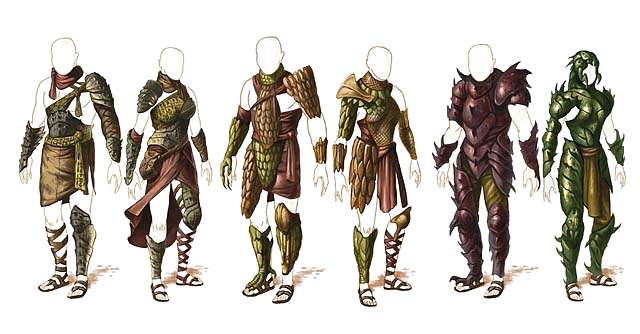
\includegraphics[width=0.5\linewidth]{images/athasian_armour.png}
\end{figure}

\FloatBarrier

\begin{multicols}{2}

\subsubsection{Heavy Robes}
\label{itmamr:heavyrobes}
These are robes made of multiple layers of thick robe.

\subsubsection{Padded Armour}
\label{itmamr:padded}
Padded armour is made of heavy cloth and batting. Many Athasian warriors prefer padded armour woven from giant hair.

\subsubsection{Crodlu Leather}
\label{itmamr:crodluleather}
This armour is crafted using hardened leather from Crodlu reinforced with bone and talons.

\subsubsection{Baazrag Leather}
\label{itmamr:baazragleather}
This armour is crafted using the hardened underhide from Baazrag combined with the cheaper parts of their shell. 
Wearing this sort of armour helps in stealth related tasks.

\subsubsection{Kank Hide Armour}
\label{itmamr:kankhide}
This armour is skillfully made by interlocking hexagonal bits of a kank’s carapace.

\subsubsection{Brohg Hide Armour}
\label{itmamr:brohghide}
This armour is made from the hardened hide from a Brogh.

\subsubsection{Reaper Chitin Armour}
\label{itmamr:reaperchitin}
This chitin armour is made from the hard chitin from a Dune Reaper.

%\subsubsection{Kank Chitin Armour}
%\label{itmamr:kreenchitin}
%Thi chiitin armour is made from insect shell of a Kank.

\subsubsection{Anakore Shell Armour}
\label{itmamr:anakoreshell}
This shell armour made from interlocking shells from an Anakore, combined with the hardened leather of the underhide and their bones.

%\subsubsection{Inix Shell Armour}
%\label{itmamr:inixshell}
%This shell armour is made by weaving giant's hair around the breast shells from Inix'.

\subsubsection{Braxat Breastplate}
\label{itmamr:braxatbreastplate}
These armours are constructed using choice plates taken from Braxat.

\subsubsection{Mekillot Breastplate}
\label{itmamr:mekillotbreastplate}
These armours are constructed using choice plates taken Mekillot.

\subsubsection{Braxat Half Plate}
\label{itmamr:braxathalfplate}
These armours are constructed using choice plates taken from Braxat.

\subsubsection{Mekillot Half Plate}
\label{itmamr:mekillothalfplate}
These armours are constructed using choice plates taken Mekillot.

\subsubsection{Braxat Full Plate}
\label{itmamr:braxatfullplate}
These armours are constructed using choice plates taken from Braxat.

\subsubsection{Mekillot Full Plate}
\label{itmamr:mekillotfullplate}
These armours are constructed using choice plates taken Mekillot.

\end{multicols}


\FloatBarrier
\section{Item Attachments}

Item attachments are ways to customize weapons or armor. They include specialised
ways to upgrade or add features and to personalize your gear. Each item attachment
has a cost in ceramic pieces, and an cost in Hard Points.

\begin{multicols}{2}
\subsection{Hardpoints}
The number of hardpoints an item has is determined by its basic encumbrance value.
An item has an number of hardpoints equal to hald an items base enumbrance value
rounded up. Once an attachment is installed, the hardpoints cost of that attachment
is now considered 'in use' and cannot be used for other attachments unless the
attachment is removed.

\subsection{Installing Attachments}

Installing an attachment requires roughly an hour of work. In addition, the character
doing the installing needs to make a successful  Average (\difficulty\difficulty)
Crafting check. Failure simply means that the attachment isn't installed, and the
character needs to try again later. Failure with a \despair (not likely unless you
upgrade the check's difficulty) means that the character clumsily destroys the
attachment in the process! Success with \despair means that the installation is
successful, but the attachment may fall off or stop working at an awkward time,
depending on the item and attachment involved.

\subsection{Weapon Attachments}
\subsubsection{Balanced Hilt}
This attachment represents modifying a melee weapon’s
balance (particularly around the hilt or haft) to make it
easier to control.\\
\textbf{Use With:} This attachment can be applied to any
    weapons that use the Melee (Light) skill.\\
\textbf{Modifiers:} The weapon gains the
    \iqtyref{accurate} 1 quality, or increases any
    existing \iqtyref{accurate} quality by 1.
    (If the weapon has the \iqtyref{inaccurate} quality,
    it reduces that quality's rating by 1 to a minimum of 0,
    instead.)\\
\textbf{Hard Points Required:} 1.\\
\textbf{Cost:} 1000.\\
\textbf{Rarity:} 6.\\

\subsubsection{Counterweight}
A counterweight attached below the grip makes the
weapon easier to swing. Can only be applied to melee
weapons with the \iqtyref{cumbersome} quality.\\
\textbf{Use With:} This attachment can be applied to any
    melee weapon with the \iqtyref{cumbersome} quality.\\
\textbf{Basic Modifiers:} Reduces the \iqtyref{cumbersome} rating by 1.
\textbf{Modification Options:} Reduce Enumbrance by 1 to a
minimum of 1.
\textbf{Hard Points Required:} 1.\\
\textbf{Cost:} 350.\\
\textbf{Rarity:} 5.\\

\subsubsection{Doubled}
A second blade or other striking surface is attached to the
opposite end of the weapon. The weapon now requires
two hands to wield.\\
\textbf{Use With:} This attachment can be applied to any
    melee weapon.\\
\textbf{Modifiers:} The weapon gains the  \iqtyref{linked} quality 1 or increase the \iqtyref{linked} quality by 1.\\
\textbf{Hard Points Required:} 1.\\
\textbf{Cost:} Weapon base cost, or new weapon cost, plus an additional 100cp.\\
\textbf{Rarity:} 6 or same as weapon, whichever is higher.\\

\subsubsection{Metal Weapon}
Extremely costly and difficult to produce and manufactor, metal is the holy grail
material for most items. The weapon must be crafted with this 'attachment', it
cannot be added later.\\
\textbf{Use With:} This attachment can be applied to any non-ranged weapon.\\
\textbf{Modifiers:}
    The weapon gains the \iqtyref{superior} quality.
    In addition it takes \despair\despair to break a metal weapon.
\textbf{Hard Points Required:} 1.\\
\textbf{Cost:} Cost x 2 + 2000cp.\\
\textbf{Rarity:} 10.\\

\subsubsection{Paired Weapon}
This attachment represents modifying a melee weapon’s
balance (particularly around the hilt or haft) to make it
easier to control.\\
\textbf{Use With:} Any one-handed weapons\\
\textbf{Modifiers:} Applied to two weapons; reduce Advantage to hit with secondary weapon when two-weapon fighting by one.\\
\textbf{Hard Points Required:} 1 (For each weapon).\\
\textbf{Cost:} 500.\\
\textbf{Rarity:} 3.\\

\subsubsection{Obsidian Weapon}
Obsidian weapons are sharper than stone, bone and chitin weapons. However
this comes at a cost by being even more fragile. The weapon must be crafted
with this 'attachment', it cannot be added later.\\
\textbf{Use With:} This attachment can be applied to any non-ranged weapon.\\
\textbf{Modifiers:}
    The weapon gains the \iqtyref{vicious} quality.\\
    The weapon breaks on a \threat\threat or \despair instead of \threat\threat\threat of the normal Athasian weapons.
\textbf{Hard Points Required:} 1.\\
\textbf{Cost:} Cost x 1.5.\\
\textbf{Rarity:} 6.\\

\subsubsection{Razor Edge}
This attachment represents sharpening a blade to
a razor edge, then reinforcing or treating that edge
so that it can withstand repeated blows.\\
\textbf{Use With:} This attachment can be applied to any close
    combat weapon that has a blade.\\
\textbf{Modifiers:} The weapon gains the \iqtyref{pierce} 2 quality, or
    increases any existing \iqtyref{pierce} quality by 1. The weapon
    also decreases its Crit rating by 1, to a minimum of 1.\\
\textbf{Hard Points Required:} 1.\\
\textbf{Cost:} 1250.\\
\textbf{Rarity:} 6.\\

\subsubsection{Recurve Limbs}
Making the limbs of a bow or crossbow curve away
from the wielder increases the penetrating power of
the bow's shots, even if it also makes the bow larger and
more difficult to wield.\\
\textbf{Use With:} This attachment can be applied to any bow
    or crossbow.\\
\textbf{Modifiers:} The weapon gains the \nameref{iqty:pierce} 2 quality, or
    increases any existing \nameref{iqty:pierce} quality by 1. The weapon
    also gains the \nameref{iqty:unwieldy} 2 quality, or increases any
    existing \nameref{iqty:unwieldy} quality by 1.\\
\textbf{Hard Points Required:} 1.\\
\textbf{Cost:} 300.\\
\textbf{Rarity:} 4.\\

\subsubsection{Serrated Edge}
Adding jagged sawteeth to a bladed weapon means the
wounds it makes are particularly brutal and damaging.\\
\textbf{Use With:} This attachment can be applied to any close
    combat weapon that has a blade.\\
\textbf{Modifiers:} The weapon gains the \iqtyref{vicious} 1 quality, or
    increases any existing \iqtyref{vicious} quality by 1.\\
\textbf{Hard Points Required:} 1.\\
\textbf{Cost:} 75.\\
\textbf{Rarity:} 2.\\


\subsection{Armor Attachments}
\subsubsection{Deflective Plating}
This attachment applies angled plates or mildly reflec-
tive surfaces to help deflect incoming ranged attacks.\\
\textbf{Use With:} This attachment can be applied to any armor.\\
\textbf{Modifiers:} Wearer increases their ranged defense by 1.\\
\textbf{Hard Points Required:} 1.\\
\textbf{Cost:} 450.\\
\textbf{Rarity:} 4.\\

\subsubsection{Gilded}
Though it serves no practical purpose, many nobles like to adorn their armor with gold leaf. It certainly makes the wearer seem impressive, but acts as a lure for every bandit within eyesight.\\
\textbf{Use With:} This attachment can be applied to any armor.\\
\textbf{Modifiers:} While wearing this armor, your character adds \boost to Charm, Negotiation, and Leadership checks.\\
\textbf{Hard Points Required:} 0.\\
\textbf{Cost:} 600.\\
\textbf{Rarity:} 7.\\

\subsubsection{Intimidating Visage}
Warriors from many cultures paint their armor or add
imposing face masks to intimidate opponents.\\
\textbf{Use With:} This attachment can be applied to any armor.\\
\textbf{Modifiers:} When wearing this armor, the user adds\\
\success to Coercion checks they make, and automatic \failure to
    Charm checks they make.\\
\textbf{Hard Points Required:} 0.\\
\textbf{Cost:} 125.\\
\textbf{Rarity:} 63\\

\subsubsection{Metal Armor}
Extremely costly and difficult to produce and manufactor, metal is the holy grail
material for most items.\\
\textbf{Use With:} This attachment can be applied to any armor with a soak rating above Hardened Leather Armor.\\
\textbf{Modifiers:} Metal Armour lose the \iqtyref{fragile} quality.
    In addition it takes \despair\despair to break a metal armor.
    However, metal armor is generally also more cumbersome. An armor with the Metal
    Armor qualifier adds 2 to its Encumbrance rating.\\
\textbf{Hard Points Required:} 2.\\
\textbf{Cost:} 10000.\\
\textbf{Rarity:} 10.\\

\subsubsection{Pockets. Lots of Pockets}
Who doesn’t love pockets? Especially common with the more unsavoury sorts. Also wizards.\\
\textbf{Use With:} This attachment can be applied to any soft armour such as leather or robes.\\
\textbf{Modifiers:} While wearing this armour, the user can carry three encumbrance 1 items at no penalty to encumbrance. These items must be no larger than the average dagger.\\
\textbf{Hard Points Required:} 1.\\
\textbf{Cost:} 400.\\
\textbf{Rarity:} 5\\

\subsubsection{Reinforced Plating}
This attachment represents adding extra layers of armor
or using stronger materials to reinforce the armor.\\
\textbf{Use With:} This attachment can be applied to any armor
    that uses hardened plates for protection.\\
\textbf{Modifiers:} The armor gains the Reinforced quality. The
    armor also increases its encumbrance by 1.\\
\textbf{Hard Points Required:} 2.\\
\textbf{Cost:} 8000.\\
\textbf{Rarity:} 7.\\

\subsubsection{Spikes}
This attachment represents adding Sharp spikes to the armor.
Often made from obsidian or sharpened bone, these hazardous
spikes can cause nasty cuts.
\textbf{Use With:} This attachment can be applied to any armor\\
\textbf{Modifiers:} If your character is targeted by a melee
    combat check while wearing this armor, you may spend
    \threat\threat\threat or \despair to cause the attacker to suffer 3 wounds.
\textbf{Hard Points Required:} 1.\\
\textbf{Cost:} 400.\\
\textbf{Rarity:} 2.\\


\end{multicols}

\FloatBarrier
\section{Goods and Services}
\subsubsection{Adventuring Gear}
\begin{table*}[!htb]
\small\caption{Adventuring Gear}
\begin{GenesysTable}{X l l l}
Name                              & Encum & Price & Rarity \\
\nameref{advitm:backpack}         & 0     & 10cp  & 2      \\
Bedroll                           & 2     & 1cp   & 1      \\
Bottle, glass                     & 1     & 10cp  & 1      \\
\nameref{advitm:caltrops}         & 1     & 5cp   & 3      \\
Candle                            & 0     & 10bit & 0      \\
Canvas (m\textsuperscript{2})     & 1     & 1cp   & 1      \\
Chain (3m)                        & 2     & 500cp & 8      \\
Chalk, 1 piece                    & 0     & 5bit  & 1      \\
\nameref{advitm:crowbar}          & 1     & 2cp   & 8      \\
Firewood (per day)                & 1     & 2cp   & 2      \\
Flask (empty)                     & 1     & 1cp   & 1      \\
\nameref{advitm:grapplinghook}    & 1     & 5cp   & 2      \\
Hammer                            & 1     & 3cp   & 0      \\
Hourglass                         & 1     & 125cp & 4      \\
\nameref{advitm:ink}              & 0     & 100cp & 6      \\
Inkpen                            & 0     & 10cp  & 6      \\
Jug, clay                         & 1     & 1cp   & 0      \\
Ladder, 3m                        & 5     & 1cp   & 1      \\
\nameref{advitm:lamp_common}      & 1     & 1cp   & 1      \\
\nameref{advitm:lantern_bullseye} & 1     & 65cp  & 3      \\
\nameref{advitm:lantern_hooded}   & 1     & 30cp  & 2      \\
\nameref{advitm:lock}             & 0     & 750cp & 8      \\
\nameref{advitm:manacles}         & 1     & 300cp & 8      \\
Mirror                            & 0     & 50cp  & 3      \\
Mug/Tankard, clay                 & 1     & 1cp   & 0      \\
\nameref{advitm:oil}              & 1     & 1cp   & 1      \\
Parchment (sheet)                 & 0     & 4cp   & 3      \\
Pick, miner's                     & 2     & 15cp  & 1      \\
Pitcher, clay                     & 1     & 1cp   & 0      \\
Pouch, belt (empty)               & 0     & 5cp   & 0      \\
Rations, trail (per day)          & 0     & 3cp   & 0      \\
\nameref{advitm:ram}              & 4     & 10cp  & 6      \\
\nameref{advitm:rope_hemp}        & 1     & 5cp   & 1      \\
\nameref{advitm:rope_silk}        & 1     & 50cp  & 3      \\
Sealing wax                       & 0     & 5cp   & 0      \\
Sewing needle                     & 0     & 3cp   & 1      \\
Shovel or spade                   & 2     & 10cp  & 0      \\
Signal whistle                    & 0     & 4cp   & 1      \\
Sledge                            & 2     & 5cp   & 4      \\
Soap (per 500g.)                  & 0     & 3cp   & 1      \\
Tent                              & 2     & 50cp  & 2      \\
\nameref{advitm:torch}            & 1     & 1cp   & 0      \\
\nameref{advitm:vial}             & 1     & 5cp   & 0      \\
Waterskin                         & 1     & 5cp   & 0      \\
Whetstone                         & 0     & 1cp   & 1      \\
\end{GenesysTable}
\end{table*}
\begin{multicols}{2}

\paragraph{Backpack} \label{advitm:backpack}
Backpacks increase the characters encumbrance by 4.

\paragraph{Caltrops} \label{advitm:caltrops}
A caltrop is a four-pronged metal spike crafted so that
one prong faces up no matter how the caltrop comes to
rest. You scatter caltrops on the ground in the hope that
your enemies step on them or are at least forced to slow
down to avoid them. One 1kg bag of caltrops
covers an area 0.5m\textsuperscript{2}.\\
Each time a creature moves into an area covered by
caltrops (or spends a round fighting while standing in
such an area), it runs the risk of stepping on one. Make
an attack roll for the caltrops with no ranks, against the
creature. For this attack defense bonuses do not count. If
the creature is wearing shoes or other footwear, add a
\setback. If the attack succeeds, the creature has stepped on a
caltrop. The target suffers 1 Wound, and the creature
applies the \textit{Hamstrung Critical (The target loses their
free maneuver until this critical is healed)}. This
Daunting (\difficulty\difficulty\difficulty\difficulty)
Brawn check upgrade the
movement penalty lasts for 24 hours, until the critical is
successfully treated, or until it receives at least 1 point
of magical healing.\\
Caltrops may not work against unusual opponents.

\paragraph{Chain} \label{advitm:chain}
A chain. Made from metal, they are rare items, often used to
restrict the movement of arena beasts.
It can be burst with a Formidable
(\difficulty\difficulty\difficulty\difficulty\difficulty)
Brawn check.

\paragraph{Crowbar} \label{advitm:crowbar}
A bar-like object, often made from Mekillot bone, used to
force things open.\\
A crowbar grants a \boost on Athletics checks made to force
open a door or chest. If used in combat, treat a crowbar
as a small improvised weapon.

\paragraph{Grappling Hook} \label{advitm:grapplinghook}
Throwing a grappling hook requires a
Ranged or Coordination check. The difficulty is based on
the range, Medium range being its maximum range.

\paragraph{Ink, 28gr} \label{advitm:ink}
Ink in colors other than black costs twice as much.

\paragraph{Jug, Clay} \label{advitm:jug}
This basic jug is fitted with a stopper and holds 4 liters of liquid.

\paragraph{Lamp, Common} \label{advitm:lamp_common}
A lamp illuminates a Short Range area. A lamp burns
for 6 hours on one pint of oil. You can carry a lamp in
one hand.

\paragraph{Lantern, Bullseye} \label{advitm:lantern_bullseye}
A bullseye lantern provides light up to medium range in
cone. A lantern burns for 6 hours on one pint of oil. You
can carry a lantern in one hand.

\paragraph{Lantern, Hooded} \label{advitm:lantern_hooded}
A hooded lantern illuminates a short range area. A
lantern burns for 6 hours on one pint of oil. You can
carry a lantern in one hand.
This lantern is encased in a more protective cover.
Add a s to any check to put out this light by means of
water or wind.

\paragraph{Lock} \label{advitm:lock}
Daunting (\difficulty\difficulty\difficulty\difficulty) Skulduggery check

\paragraph{Manacles} \label{advitm:manacles}
Restraints made from metal, these things are used only for
the most dangerous of enemies or by the most rich slave- or
bounty-hunters.\\
Manacles can bind a Medium creature. To slip free, a
creature must roll a Formitable (\difficulty\difficulty\difficulty\difficulty)
Coordination Check.  Breaking the manacles requires a
Daunting (\difficulty\difficulty\difficulty\difficulty) Brawn check.
Most manacles have locks; add the cost of the lock
to the cost of the manacles.
For the same cost, you can buy manacles for a Small
creature. For a Large creature, manacles cost 10 times
the indicated amount, and for a Huge creature, 100
times the indicated amount. Gargantuan, Colossal, Tiny,
Diminutive, and Fine creatures can be held only by
specially made manacles, which cost at least 100 times
the indicated amount.
The checks to escape all get setbacks.

\paragraph{Oil, 1 pint flask} \label{advitm:oil}
A pint of oil burns for 6 hours in a lantern or lamp.
You can also use a flask of oil as a splash weapon.
With the proper skill you can use oil as an attack
Roll an Average (\difficulty\difficulty) Alchemy check,
with a base damage of 3 and a burn 1 quality. You
can pour a pint of oil on the ground to cover an
area 0.5m\textsuperscript{2}, provided that the surface is
smooth. If lit,the oil burns for 2 rounds and deals
the base damage of the weapon to each creature in
the area.

\paragraph{Ram, Portable} \label{advitm:ram}
This iron-shod wooden beam gives you an \boost on
Brawn checks made to break open a door and
allows a second person to help give you \boost\boost
instead of one.

\paragraph{Rope, Hemp (20m)} \label{advitm:rope_hemp}
This rope can be burst with a Hard (\difficulty\difficulty\difficulty)
Brawn check.

\paragraph{Rope, Silk (20m)} \label{advitm:rope_silk}
This rope can be burst with a Hard (\difficulty\difficulty\difficulty\setback)
Brawn check.

\paragraph{Torch} \label{advitm:torch}
A torch burns for 1 hour, shedding lighting on
everything within Short Range.
If a torch is used in combat, treat it as a small
improvised weapon with a \iqtyref{burn} 1 quality.

\paragraph{Vial} \label{advitm:vial}
A vial is made out of glass and holds 1 ounce of liquid.

\end{multicols}
\subsubsection{Alchemical Items}
\begin{table*}[!htb]
\small\caption{Alchemical Items}
\begin{GenesysTable}{X l l l}
Name                              & Encum & Price & Rarity \\
\nameref{alcitm:acid}             & 0     & 50    & 2      \\
\nameref{alcitm:alchemistsfire}   & 0     & 100   & 2      \\
\nameref{alcitm:antitoxin}        & 0     & 250   & 3      \\
\nameref{alcitm:healingpoultrice} & 0     & 10    & 2      \\
\nameref{alcitm:smokestick}       & 0     & 100   & 2      \\
\nameref{alcitm:tanglefootbag}    & 1     & 250   & 3      \\
\nameref{alcitm:thunderstone}     & 0     & 150   & 3      \\
\nameref{alcitm:tindertwig}       & 0     & 5     & 0      \\
\end{GenesysTable}
\end{table*}
\begin{multicols}{2}

\paragraph{Acid} \label{alcitm:acid}
You can throw a flask of acid as a weapon with an
Ranged light or Alchemy combat check with a base
damage of 6 acid damage, with a range of short, and
\iqtyref{blast} 3, \iqtyref{sunder}.
It can also be used to damage a lock beyond repair.

\paragraph{Alchemist's Fire} \label{alcitm:alchemistsfire}
You can throw a flask of alchemist’s fire as a weapon
with an Ranged light or Alchemy combat check with
a base damage of 6 fire damage, with a range of short,
and \iqtyref{blast} 3, \iqtyref{burn} 2 .

\paragraph{Antitoxin} \label{alcitm:antitoxin}
If you drink a vial of antitoxin, you get an upgrade on
your Resilience check against poison for 1 hour.

\paragraph{Healing Poultrice} \label{alcitm:healingpoultrice}
A healing poultrice is a soft moist mass, often heated and
medicated, that is spread on cloth over the skin to treat an
aching, inflamed or painful part of the body. It can be used
on wounds such as cuts. It is a one-use item and provide a \boost
to medicine checks to treat cuts, bruises and minor ailments.

\paragraph{Smokestick} \label{alcitm:smokestick}
This alchemically treated wooden stick instantly creates
thick, opaque smoke when burned. The smoke fills a
short range radius, The stick is consumed after 1 round,
and the smoke dissipates naturally after 1 minute.\\
A creature that is engaged range with the fog adds
\setback on Perception, Vigilance, and all combat skill
checks. Creatures farther away looking or targetting into
the mist add \setback\setback to their Perception, Vigilance,
and all combat skill checks.

\paragraph{Tanglefoot Bag} \label{alcitm:tanglefootbag}
tanglefoot bag is a small sack filled with tar, resin
and other sticky substances. When you throw a
tanglefoot bag at a creature roll a Ranged Light or
Alchmey combat check. This attack has a range of
short, does no damage. If successful the attack is treated
as if the wielder activated an \iqtyref{ensnare} 5 quality. The
bag comes apart and goo bursts out, entangling the
target and then becoming tough and resilient upon
exposure to air.

\paragraph{Thunderstone} \label{alcitm:thunderstone}
You can throw this stone as a weapon with an Ranged(Light) or
Alchemy combat check with a range of short and deals no damage.
When it strikes a hard surface (or is struck hard), it creates
a deafening bang that is treated as a sonic attack. Each creature
within short range of where it went off must make an Average
(\difficulty\difficulty) Resilence check or be deafened for 1
hour. A deafened creature, in addition to the obvious effects,
takes \setback\setback on initiative rolls and has a \setback
when casting a spell

\paragraph{Tindertwig} \label{alcitm:tindertwig}
The alchemical substance on the end of this small,
wooden stick ignites when struck against a rough
surface. Creating a flame with a tindertwig is much
faster than creating a flame with flint and steel (or a
magnifying glass) and tinder. Lighting a torch with a
tindertwig is a maneuver (rather than an action), and
lighting any other fire with one is a maneuver.

\end{multicols}
\subsubsection{Tools and Kits}
\begin{table*}[!htb]
\small\caption{Tools and Kits}
\begin{GenesysTable}{X l l l}
Name                             & Encum & Price & Rarity \\
\nameref{kititm:alchemistslab}   & 5     & 50    & 6      \\
\nameref{kititm:artisanstools}   & 4     & 150   & 0      \\
\nameref{kititm:climberskit}     & 1     & 50    & 2      \\
\nameref{kititm:disguisekit}     & 2     & 100   & 4      \\
\nameref{kititm:healerskit}      & 1     & 100   & 2      \\
\nameref{kititm:thievestools}    & 0     & 100   & 7      \\
\end{GenesysTable}
\end{table*}
\begin{multicols}{2}

\paragraph{Alchemist's Lab} \label{kititm:alchemistslab}
This lab is used for making alchemical items, and
provides a \boost on Alchemy checks pertaining to crafting.

\paragraph{Artisan's Tools} \label{kititm:artisanstools}
These special tools include the items needed to pursue
any craft. Without them, you have to use improvised
tools and take a \setback on Crafting checks), if you
can do the job at all.

\paragraph{Climber's Kit} \label{kititm:climberskit}
These crampons, pitons, ropes, and tools give you a \boost check.
on Athletics checks when Climbing.

\paragraph{Disguise Kit} \label{kititm:disguisekit}
The kit is the perfect tool for disguise and provides a \boost
on Deception checks. A disguise kit is exhausted after
10 uses.

\paragraph{Healer's Kit} \label{kititm:healerskit}
This collection of bandages and herbs provides a \boost on
Medicine checks. A healer's kit is exhausted with
\threat\threat\threat or \despair.

\paragraph{Thieves's Tools} \label{kititm:thievestools}
This kit contains lockpicks and other tools you need to
use the Skulduggery skill. Without these tools, you must
use improvised tools, and you take a \setback on Skulduggery
checks, with these tools you get a \boost to a lock or a latch.

\end{multicols}

\hrulefill
\subsubsection{Mounts}
\begin{multicols}{2}

Athasians have domesticated a variety of mounts. The
most common are presented below. More unusual
steeds, such as giant ants, spiders, drakes, and
wyverns can be found, but not easily or cheaply.

\begin{table}[H]
\centering
\small\caption{Mounts}
\begin{GenesysTable}{X l l l l}
Name                       & Speed & Encumbrance & Price    & Rarity \\
\nameref{itmmnt:crodlu}    & 7     & 10          & 2250cp   & 3      \\
\nameref{itmmnt:warcrodlu} & 7     & 10          & 10000cp  & 6      \\
\nameref{itmmnt:erdlu}     & 7     & 10          & 750cp    & 2      \\
\nameref{itmmnt:kank}      & 7     & 10          & 8400cp   & 7      \\
\nameref{itmmnt:inix}      & 5     & 10          & 20000cp  & 5      \\
\nameref{itmmnt:mekillot}  & 6     & 10          & 40000cp  & 8      \\
\end{GenesysTable}
\end{table}

\paragraph{Crodlu}
\label{itmmnt:crodlu}
A crodlu is a large, flightless drake with a beak and
weak, clawed forelimbs that can be used to manipulate
small objects. It is a tough and aggressive hunter
in the wild. See \nameref{creature:Crodlu} for more
information.

\paragraph{War Crodlu}
\label{itmmnt:warcrodlu}
A crodlu is a large, flightless drake with a beak and
weak, clawed forelimbs that can be used to manipu-
late small objects. It is a tough and aggressive hunter
in the wild. When trained, it makes an excellent war
mount. See \nameref{creature:War Crodlu} for more information.

\paragraph{Erdlu}
\label{itmmnt:erdlu}
The erdlu is a smaller version of the crodlu. Its body
is covered in tough scales, and its folded forelimbs
sprout useless wings. Hardy and fast, this drakelike
creature is a fine riding beast for a Silhoutte 0 rider.
It is too skittish to be trained for war, however. See
\nameref{creature:Erdlu} for more information.

\paragraph{Kank}
\label{itmmnt:kank}
Kanks are docile insects that form hives. Each member
of the group has a role: food producer, soldier, or
the brood queen. The kank soldier can be trained for
riding and battle. See \nameref{creature:Kank} for
more information.

\paragraph{Inix}
\label{itmmnt:inix}
An inix, also called a dune behemoth, is a long, low-
slung reptile with bony plates on its back. It is strong
and spirited. An inix rarely eats anything as large as
a humanoid, but it does not shy away from a fight. See
\nameref{creature:Inix} for more information.

\paragraph{Mekillot}
\label{itmmnt:mekillot}
These massive creatures serve as draft animals
given their tremendous pulling strength. They are
aggressive, however, and have been known to turn
on handlers. See \nameref{creature:Mekillot} for
more information.

\end{multicols}

\hrulefill
\subsection{Magical and Psionics Gear}
\begin{multicols}{2}

\begin{table}[H]
\centering
\small\caption{Magic and Psionic Gear}
\begin{GenesysTable}{X l l l}
Name                                         & Encumbrance & Price & Rarity \\
\nameref{itmmgc:healingfruit}                & 0           & 30    & 5 \\
\nameref{itmmgc:spellcomponentpouch}         & 1           & 50    & (I) 3 \\
\end{GenesysTable}
\end{table}

\paragraph{Healing Fruit} \label{itmmgc:healingfruit}
Healing Fruits are fruit grown from magical infused fruit trees.
While using any fruit is possible, often pears are most common.
While they are great for infusing a living body with healing,
their effects do diminish quite fast. The first healing fruit
eaten on a day grants 5 healing, the second eaten the same day
4 healing and so forth.

\paragraph{Spell Component Pouch}
\label{itmmgc:spellcomponentpouch}
A spell component pouch contains the spell components neccesary to cast Primal
Spells. A spell component pouch can contain one or more components, which must
be bought seperately or be sought out. An spell component is empty when a \despair
is used to 'damage' the spell component using a magic skill check, in which case
the spell component must either be bought again or sought after anew. See~\tref{table:spell_components} for a list for Spell Components.

\textit{TODO: Create better spell component names, and are they balanced?}

\end{multicols}

\begin{table}[htb]
\centering
\small\caption{Spell Components}
\begin{GenesysTable}{l l l X}
Component   & Cost      & Rarity    & Description \\
S1          & (I) 800   & 7         & When casting an conjure spell to summon an elemental,
                                            adding the Summon Ally effect does not increas its
                                            difficulty. In addition, the creature remains
                                            summoned untill the end of the encounter without
                                            your character having to use a concentrate manouvre.\\
S2          & (I) 400   & 6         & When casting a spell, adding the first Range effect added
                                            to the spell does not increase the spell's difficulty.\\
S3          & (I) 1000  & 9         & When casting a spell, the caster may count any additional
                                            \success beyond those needed to hit as \advantage\advantage\advantage
                                            required to activate any added effect.\\
%S4          &          & Rarity     & Attack spells cast by the user increase their base damage by 4.\\
\end{GenesysTable}
\label{table:spell_components}
\end{table}


\section{Selling and Trading}\label{chap:sec:trading}

This Section is extremely experimental.\\
\\
In some cases, the PCs might wish to engage in trade, buying multiple items at one
location and then selling them at another location where they are rarer. We generally
advise that you handle this narratively. However, if your GM wishes to use some
mechanical guidelines for this process, we’ve provided some basic rules that cover trading.\\
\\
Trade works the same whether with black-market items or with legal items. Selling
either type of item follows the rules listed previously with the caveat that trading
in legal items requires a Negotiation check, while trading in illegal items requires a
Streetwise check. However, when determining the sell price based on the success of the
Negotiation or Streetwise check, first multiply the cost of the item by the difference
between the item's rarity where it was bought and its rarity where it is to be sold,
referring to \tableref{equipment-rarity-modifiers} and \tableref{equipment-rarity-costs}.
Then take the new, increased cost and determine the sell price by the results of the
Negotiation or Streetwise check.\\
\\
Of course, these rules do not account for all sorts of details, such as buying in bulk,
marketing and advertising, and myriad other factors that may affect prices.\\
\\
This is why the rules for buying, selling, and trading are all modifiable by the GM and
subject to their judgement. It is also important to note that these rules only apply when
engaging in commercial trade. So, if your group sells a load of guns in a town, then
later your character buys one of those guns in that town, they’re going to have to pay
usual, listed price for the gun. The final thing to remember is that your GM always has the
final say on what can be sold, where it can be sold, and how much it can be sold for.
Because this isn't likely to be a major part of the game, we deliberately made a system
that is simple and doesn't account for a lot of the variables that would normally matter
when trying to sell an item.

\begin{table*}[!htb]
\begin{GenesysTable}{Selling and Trading Modifiers}{trading-modifiers}{ =l +X}
Difficulty Or Modifier                 & Result Options\\
\difficulty                            & Standard Selling Price of X 0.25\%\\
\difficulty\difficulty                 & Increased Selling Price of X 0.50\%\\
\difficulty\difficulty\difficulty      & High Selling Price of X 0.75\%\\
Each \advantage\advantage or \triumph  & Change the price by 10\% in favour of the active players.\\
Each \success                          & Change the price by  5\% in favour of the active players.\\
Each \threat\threat or \despair        & Change the price by 10\% against the active players.\\
Each \failure                          & Change the price by  5\% against the active players.\\
\triumph                               & The goods are of exceptional quality. The merchant will gladly take them of your hands and owes you a favour!\\
\despair                               & The other party is simply not interrested in making a deal, and the players should find another merchant to deal with. Increase the difficulty as normal.\newline
                                         Fake goods! The merchant wil get angry by this swindling attempt!\\
\boost                                 & Minor positive local modifer for the trade.\\
\setback                               & Minor negative local modifer for the trade.\\
+1 \difficulty                         & Each time the players decide not to go through with a deal after an negotiation, the difficulty to retry with a different merchant in the same city increases by one, for the duration of one week.\\
\end{GenesysTable}
\end{table*}

\begin{table*}[!htb]
\begin{GenesysTable}{Trading Cost and Rarity Increase}{trading}{ =l +X +X +X +X +X +X +X +X}
Item             & Base Cost per 1 enc & Balic & Draj & Gulg & Nibenay & Raam & Tyr & Urik\\
Ale              & 20cp                &   +1  &   +2 &  +1  &    +1   &   0  &   0 &   +1\\
Amber            & 8000cp              &   +1  &   +2 &   0  &    +2   &  +1  &   0 &   +1\\
Beer             & 50cp                &   +1  &   +1 &   0  &    +1   &  +2  &  +1 &   +1\\
Bronze           & 700cp               &   +2  &   +2 &  +1  &    +1   &  +1  &   0 &   +2\\
Candy            & 1cp                 &   +1  &   +1 &  +2  &    +2   &   0  &   0 &   +1\\
Ceramics         & 50cp                &   +2  &   +1 &  +1  &    +2   &   0  &   0 &   +1\\
Chalk            & 1cp                 &   +1  &   +2 &  +2  &    +1   &   0  &   0 &    0\\
Chitin           & 400cp               &   +1  &   +2 &  +2  &     0   &  +1  &  +1 &   +2\\
Cider            & 30cp                &   +2  &   +1 &   0  &    +1   &  +2  &  +1 &   +1\\
Cinnabar         & 1600cp              &   +2  &   +1 &   0  &    +2   &  +1  &  +1 &    0\\
Cloth            &                     &       &      &      &         &      &     &    \\
  Common         & 50cp                &   +1  &   +1 &   0  &    +1   &  +1  &  +2 &   +2\\
  Fine           & 100cp               &   +2  &    0 &  +2  &    +1   &  +1  &  +1 &   +1\\
  Rich           & 1000cp              &   +1  &    0 &  +2  &    +2   &   0  &  +1 &    0\\
Coal             &                     &   +1  &   +1 &   0  &    +1   &  +2  &  +2 &    0\\
Copper           & 500cp               &   +2  &   +2 &  +2  &     0   &  +1  &   0 &   +2\\
Cosmetics        & 1600cp              &   +2  &   +1 &  +1  &    +1   &   0  &   0 &    0\\
Cotton           & 20cp                &   +1  &   +2 &  +1  &    +1   &   0  &   0 &   +2\\
Dyes/Pigments    & 1600cp              &   +1  &   +2 &   0  &    +1   &   0  &  +1 &   +2\\
Feathers         &                     &       &      &      &         &      &     &     \\
  Common         & 1cp                 &   +1  &   +2 &   0  &    +1   &  +1  &   0 &    0\\
  Rare           & 50cp                &   +2  &   +2 &   0  &    +1   &   0  &   0 &    0\\
Figs             & 10cp                &   +2  &   +1 &   0  &    +1   &  +2  &  +2 &   +1\\
Fruits           & 20cp                &   +1  &   +1 &   0  &    +1   &  +2  &  +2 &   +1\\
Furs             & 100cp               &   +2  &   +1 &  +2  &    +1   &   0  &  +1 &    0\\
Glass            & 100cp               &   +2  &   +1 &  +2  &    +1   &  +1  &   0 &   +1\\
Gold             & 50000cp             &   +1  &    0 &  +1  &    +2   &   0  &  +1 &   +1\\
Hardwood         & 150cp               &   +1  &   +2 &   0  &     0   &  +1  &   0 &   +2\\
Herbs            & 30cp                &    0  &   +1 &  +1  &    +1   &  +2  &  +2 &    0\\
Incence          & 3200cp              &   +1  &   +2 &  +1  &    +2   &   0  &  +1 &    0\\
Ink              & 640cp               &   +1  &   +2 &  +2  &    +1   &  +1  &   0 &    0\\
Iron             & 1000cp              &   +2  &   +1 &  +2  &    +1   &  +2  &   0 &   +2\\
Jade             & 100cp               &   +1  &   +1 &  +2  &    +1   &  +1  &   0 &   +1\\
Kank Nectar      & 10cp                &    0  &    0 &  +2  &    +1   &  +2  &  +2 &   +1\\
Leather          & 25cp                &    0  &    0 &  +1  &    +1   &  +2  &  +1 &   +2\\
Marble           & 40cp                &   +2  &    0 &   0  &    +1   &  +1  &  +2 &    0\\
Medicines        & 800cp               &   +1  &   +2 &  +1  &    +1   &  +2  &   0 &   +1\\
Mirrors          & 100cp               &   +1  &   +1 &  +2  &     0   &  +1  &   0 &    0\\
Nuts/Dried Fruit & 10cp                &   +2  &   +1 &   0  &    +1   &  +2  &  +2 &    0\\
Obsidian         & 50cp                &   +2  &   +2 &  +1  &     0   &  +2  &   0 &   +2\\
Oil              &                     &       &      &      &         &      &     &     \\
  Flabbable      & 40cp                &    0  &   +2 &  +1  &     0   &   0  &  +1 &   +2\\
  Lamp           & 2cp                 &   +1  &    0 &  +1  &    +2   &  +1  &  +1 &   +1\\
  Cooking        & 15cp                &   +1  &   +1 &   0  &     0   &  +2  &  +2 &   +1\\
Paper            & 200cp               &   +2  &   +2 &  +1  &    +1   &   0  &  +1 &   +1\\
Perfume          & 800cp               &   +2  &   +1 &  +1  &    +2   &  +1  &   0 &    0\\
Resins           & 600cp               &   +1  &    0 &  +1  &    +1   &  +1  &  +2 &    0\\
Rice             & 10cp                &   +1  &   +2 &  +1  &     0   &  +2  &  +2 &   +1\\
Rope             &                     &       &      &      &         &      &     &     \\
  Hemp           & 5cp                 &   +2  &    0 &  +1  &    +1   &  +1  &  +1 &   +1\\
  Silk           & 10cp                &   +2  &    0 &   0  &    +2   &  +1  &   0 &   +1\\
Rugs             &                     &    0  &   +2 &  +1  &    +2   &  +1  &   0 &    0\\
Salt             & 20cp                &    0  &   +1 &  +1  &    +1   &  +2  &  +2 &    0\\
Silk, raw        & 500cp               &    0  &   +1 &  +2  &    +1   &   0  &   0 &    0\\
Silver           & 5000cp              &    0  &   +1 &  +2  &    +1   &   0  &  +1 &   +2\\
Songbirds        &                     &    0  &   +1 &  +1  &    +2   &  +1  &   0 &    0\\
Spice            &                     &       &      &      &         &      &     &     \\
  Exotic         & 1500cp              &    0  &   +1 &   0  &     0   &  +1  &   0 &   +2\\
  Rare           & 200cp               &   +1  &   +1 &   0  &     0   &  +2  &  +1 &   +2\\
  Uncommon       & 100cp               &   +1  &   +1 &   0  &     0   &  +2  &  +1 &   +2\\
Sugar            & 4cp                 &   +1  &   +1 &   0  &    +1   &  +2  &  +2 &    0\\
Tools            & 50cp                &    0  &   +1 &  +1  &     0   &  +2  &  +1 &   +1\\
Vegetables       & 20cp                &   +1  &   +1 &  +1  &     0   &  +2  &  +2 &   +1\\
Water            & 10cp                &   +2  &   +1 &  +1  &     0   &  +2  &  +2 &   +1\\
Wax              & 70b                 &   +1  &   +1 &  +2  &    +1   &   0  &  +1 &   +1\\
Wine             & 100cp               &   +2  &   +1 &   0  &    +1   &  +2  &  +2 &    0\\
Wheat            & 50cp                &   +1  &    0 &  +1  &    +1   &  +2  &  +2 &   +1\\
\end{GenesysTable}
\end{table*}
